\section{Attacker Profile \& Victimology}

\begin{frame}[fragile]{Attacker Profile i}
  \begin{itemize}
    \item Turla is well known for its advanced custom tools and its ability to run highly targeted operations.
    \item The group is interested in collecting information from strategic people
    or organizations.
  \end{itemize}
  \begin{figure}
    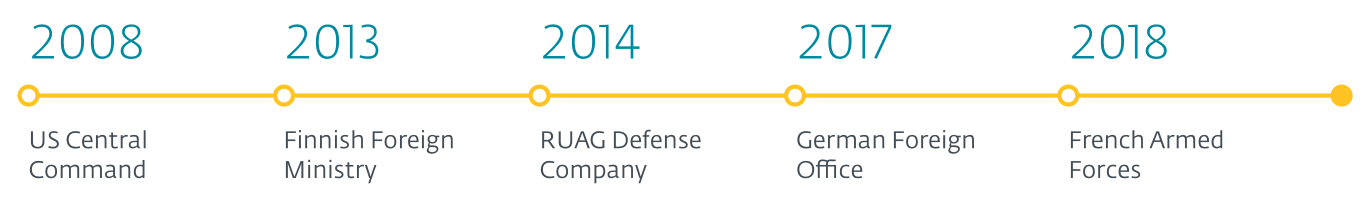
\includegraphics[width=\textwidth]{figures/timeline.PNG}
    \caption{Timeline of important attacks attributed to Turla}
  \end{figure}
\end{frame}

\begin{frame}[fragile]{Attacker Profile ii}
    \begin{itemize}
      \item The operators activity matches a typical 9-to-5 workday in the UTC+3 time zone
      \item LightNeuron is used mostly to exfiltrate data. The remaining activity is most likely dropping
      and executing tools to perform lateral movements across the local network
    \end{itemize}
    \begin{figure}
      \centering
      \subfloat[Operators working hours\label{fig:a}]{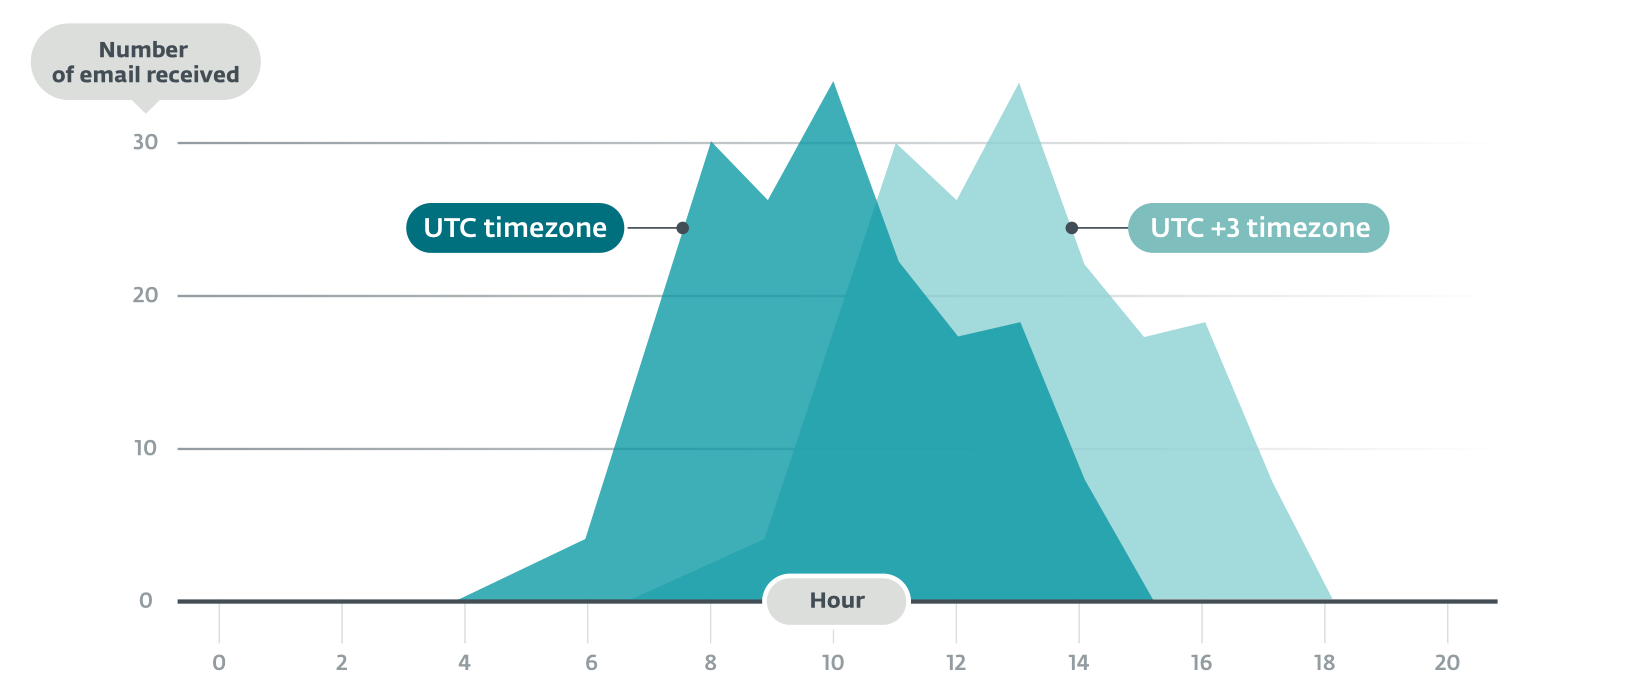
\includegraphics[height=3.5cm,width=5.5cm]{figures/attacker_timeline.PNG}}\qquad
      \subfloat[Distribution of the backdoor commands used by the operators\label{fig:b}]{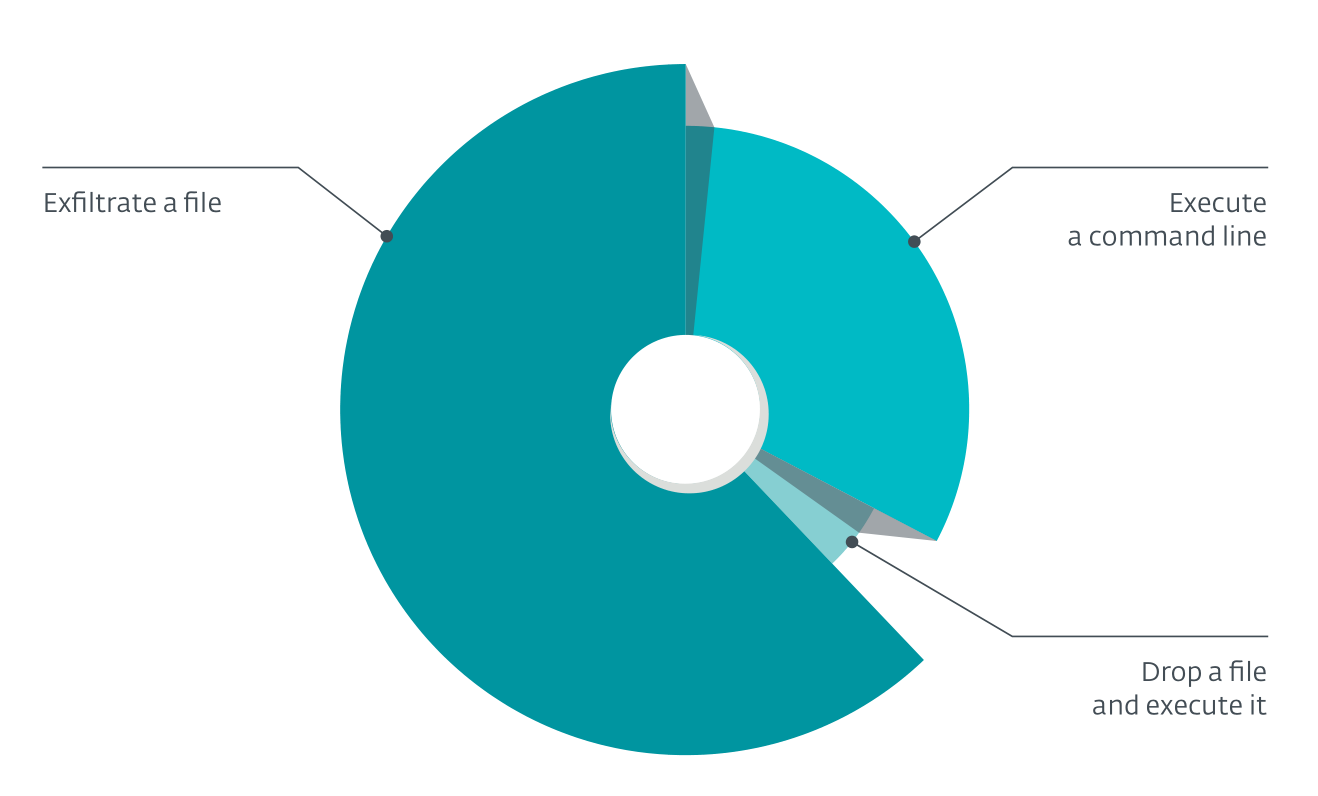
\includegraphics[height=3.5cm,width=4.6cm]{figures/commands_distrib.PNG}}
    \end{figure}
\end{frame}

\begin{frame}[fragile]{Victimology}
  According to ESET, LightNeuron development started before 2014; even if the development occurred
several years ago, LightNeuron is still used in recent compromises. These targets are in line with traditional Turla targets:
\begin{figure}
  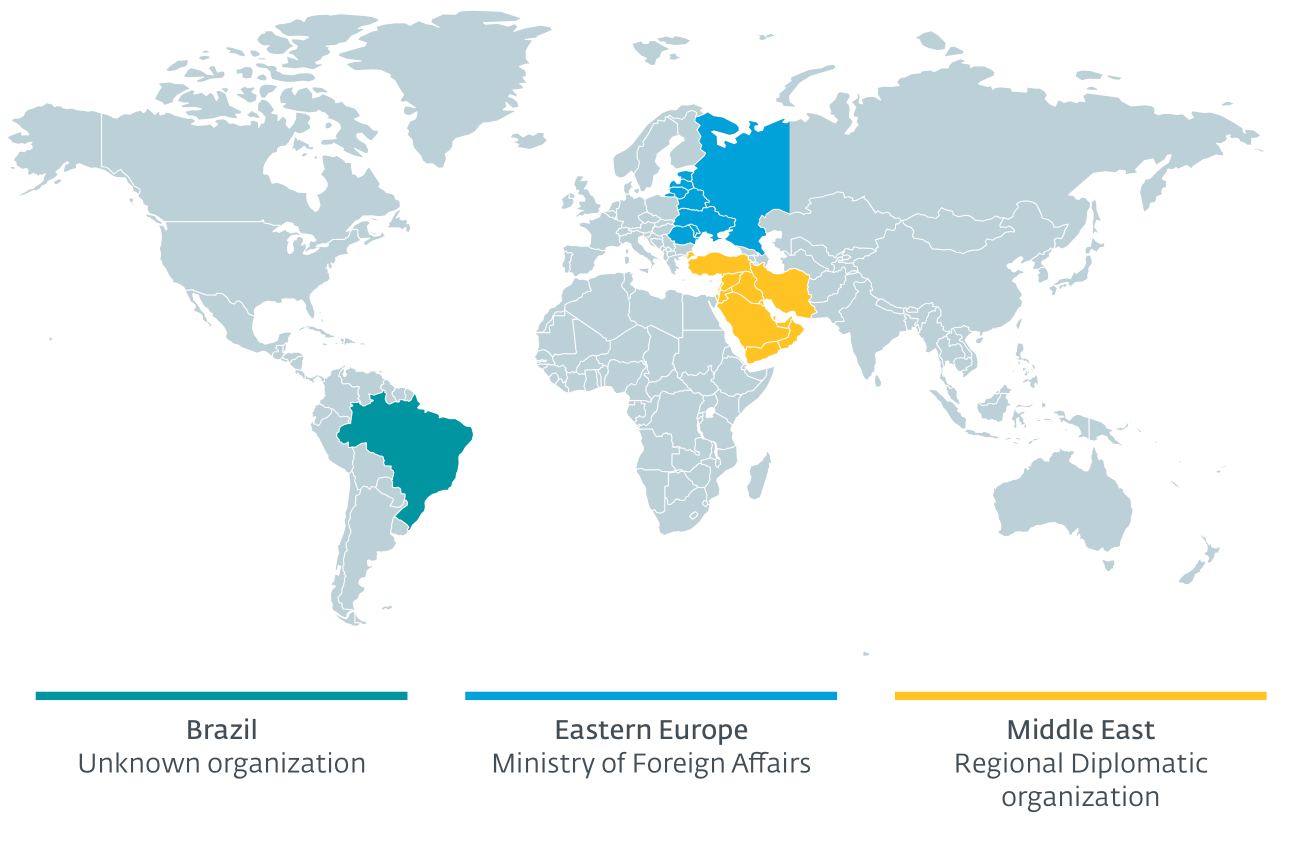
\includegraphics[width=8cm]{figures/map.PNG}
  \caption{Map of known LightNeuron victims}
\end{figure}
\end{frame}